
\subsection{Experimentation}
\label{subsec:experiments2}

We highlight the improvements brought to gossiping protocols on a real-life use
case concerning decentralized collaborative editing in browsers.  These
experiments run on Grid'5000 testbed and involve uptill 600 browsers
simultaneously writing a document. Using \SPRAY, we expect a traffic
logarithmically scaling compared to the network size, along with a
polylogarithmic growth brought by the real-time editor itself. The code of
\CRATE is hosted on the Github
platform\footnote{\url{https://github.com/Chat-Wane/CRATE}}.

\vspace{-7pt}
\paragraph{CRATE on network of browsers}

\begin{figure}
  \centering
  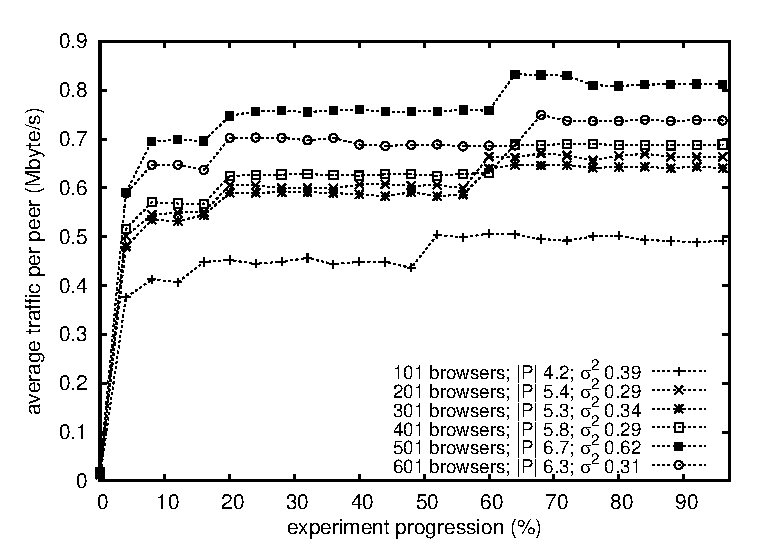
\includegraphics[width=0.49\textwidth]{img/traffic.eps}
  \caption{\label{fig:traffic}Average traffic per second.}
\end{figure}

\begin{asparadesc}
\item [Objective:] To show the influence of \SPRAY's adaptiveness over the
  traffic generated by decentralized editors running on a network of browsers.
\item [Description:] Experiments run on Grid'5000 where machines host 5 browsers
  each. Browsers open \CRATE and connect to an editing session through a
  signaling server.  Runs comprise from 101 browsers to 601 browsers with 100
  browsers increments, i.e., 6 different runs.  The first editor creates the
  editing session which is progressively joined by the other writers (1 joiner
  per 5 seconds). Each member starts sharing the access to the editing session
  as soon as it joins it. Hence, outsiders join the network through one of them
  chosen at random. Once all peers have joined the editing session, they start
  inserting characters in the document. The insertion rate is 100 insertions per
  second uniformly distributed among peers. Each experiment runs during 8 hours
  of which 7 hours are dedicated to editing. The document size reaches millions
  of characters.
\item [Results:] Figure~\ref{fig:traffic} shows the average traffic per second
  of members involved in the editing session. Legend shows the average partial
  view and the variance associated with each run. As expected, we observe a
  logarithmic multiplicative factor coming from the information dissemination
  (cf. Section~\ref{subsec:gossiping}). 101 browsers have an average traffic per
  second lower than 601 browsers because the average partial view size of the
  former is lower.  On the opposite, it worth noting that using \CYCLON, the
  traffic would have been the same for all runs. Since it commonly overestimates
  partial views to accommodate with any network size, the traffic would have
  been higher (cf. Figure~\ref{fig:churn}).  Figure~\ref{fig:traffic} also shows
  that the average partial view size follows the natural logarithmic expectation
  with small error due to randomness. Figure~\ref{fig:traffic} finally shows
  that the variance remains small which indicates that the network of browsers
  reached a state where neighborhood size are balanced.
\item [Reasons:] Information dissemination uses neighborhoods to broadcast
  messages. Each member receives and forwards each message which transitively
  reach all members. Thus, the traffic depends of the message multiplied by the
  number of neighbors logarithmically scaling thanks to \SPRAY. The growth
  during each run corresponds to the polylogarithmic growth of identifiers from
  the application. Indeed, identifiers allocated by \TODO{\LSEQ are lists of
    Integers [$l_1.l_2\ldots l_k$] where $k$ is the size of the identifier. With
    incoming characters arriving, the size of the identifiers grows and the
    Integer range as well. Therefore, $l_k$ takes 1 additionnal bit to encode
    than $l_{k-1}$, leading to twice additionnal possible identifiers.}  Small
  identifiers reflect small documents. Large identifiers reflect large
  documents. At the end, documents store millions of characters.
\end{asparadesc}
